%\documentclass[class=article, crop=false]{standalone}
%\usepackage[utf8]{inputenc}
\usepackage[T1]{fontenc}
\usepackage[english]{babel}
%\usepackage[iso]{date}
\usepackage{microtype} % optional, for aesthetics
\usepackage{csquotes}
\usepackage{fontawesome}
%%%%%%%%%%%%%%%%%%%%%%%%%%%%%%%%%%%%
%			Bibliography			%
%%%%%%%%%%%%%%%%%%%%%%%%%%%%%%%%%%%%
\usepackage[backend=biber,style=numeric-comp,sorting=none,natbib=true]{biblatex}
\addbibresource{./BIB/Bibliography.bib}

%%%%%%%%%%%%%%%%%%%%%%%%%%%%%%%%%%%%
%			Hyperref				%
%%%%%%%%%%%%%%%%%%%%%%%%%%%%%%%%%%%%
\usepackage{hyperref}
\usepackage{lastpage}
\hypersetup{
	breaklinks=false,
	citecolor=red,
	colorlinks=true,
	linkcolor=red,
	menucolor=black,
	pdfauthor={Thomas Arne Hensel},
	urlcolor=blue,
	bookmarks=true
}
%%%%%%%%%%%%%%%%%%%%%%%%%%%%%%%%%%%%
%				math				%
%%%%%%%%%%%%%%%%%%%%%%%%%%%%%%%%%%%%
\usepackage{amsmath}
\usepackage{amssymb}
\usepackage{amsthm}
\usepackage{commath}
\usepackage{siunitx}
\usepackage{eulervm}
%
%%%%%%%%%%%%%%%%%%%%%%%%%%%%%%%%%%%%
%		Figures and Plotting		%
%%%%%%%%%%%%%%%%%%%%%%%%%%%%%%%%%%%%
%
%\graphicspath{{SECTIONS/GRAPHICS/}}
\usepackage[dvipsnames]{xcolor}
\usepackage{graphicx}
\usepackage{caption,subcaption}%for subfigures
\usepackage{standalone}%to separately produce standalone figures
\usepackage{import}%to import figures later
%
\usepackage{tikz}%drawings like geometries
\usetikzlibrary{calc,matrix,positioning}
\usetikzlibrary{decorations.pathmorphing,patterns}
\usepackage{tikzscale}
%
\usepackage{pgfplots}
\pgfplotsset{
    ,compat=newest%1.12
    }
\usepgfplotslibrary{groupplots}
\usepgflibrary{patterns}
\usepackage{pgfplotstable}
%%%%%%%%%%%%%%%%%%%%%%%%%%%%%%%%%%%%
%				Tables				%
%%%%%%%%%%%%%%%%%%%%%%%%%%%%%%%%%%%%
\usepackage{multirow}
\usepackage{lscape}
\usepackage{pdflscape}
\usepackage{rotating}
\usepackage{tabularx}
\usepackage{booktabs}
%%%%%%%%%%%%%%%%%%%%%%%%%%%%%%%%%%%%
%			print git-hash			%
%%%%%%%%%%%%%%%%%%%%%%%%%%%%%%%%%%%%
\usepackage{etoolbox}
\newtoggle{submissionBuild}
\settoggle{submissionBuild}{false}
\nottoggle{submissionBuild}{%
	\usepackage{gitver}
	\usepackage{soul}
	\sethlcolor{green}
}{}
%%%%%%%%%%%%%%%%%%%%%%%%%%%%%%%%%%%%
%			Headings				%
%%%%%%%%%%%%%%%%%%%%%%%%%%%%%%%%%%%%
\usepackage{fancyhdr}
\setlength{\headheight}{15pt}

\pagestyle{fancy}
%\renewcommand{\chaptermark}[1]{ \markboth{#1}{} }
%\renewcommand{\sectionmark}[1]{ \markright{#1} }

\fancyhf{}
\fancyhead[LE,RO]{\footnotesize{p. \thepage\ / \pageref{LastPage}}}
\fancyhead[RE]{\emph{ \nouppercase{\leftmark}} }
\fancyhead[LO]{\emph{ \nouppercase{\rightmark}} }
\fancyfoot[CE,CO]{\iftoggle{submissionBuild}{}{%
  	\noindent{\emph{Revision}\/}: \hl{\mbox{\#\gitVer}}
	}}


\fancypagestyle{plain}{ %
  \fancyhf{} % remove everything
  \renewcommand{\headrulewidth}{0pt} % remove lines as well
  \renewcommand{\footrulewidth}{0pt}
}
% This will set fancy headings to the top of the page. The page number will be
% accompanied by the total number of pages. That way, you will know if any page is missing.
% If you do not want this for your document, you can just use``\pagestyle{plain}``.
%
\usepackage{todonotes}
%----------------------
%       Own definitions and macros
%----------------------
%
%
%----------------------
%       Annotation
%----------------------
%
\newcommand{\blue}[1]{\textcolor{blue}{#1}}%for blue comments
%\DeclareUnicodeCharacter{FFFD}{\blue{XXXX}}%to find false displayed characters, e.g. in Bib
%%%%%%%%%%%%%%%%%%%%%%%%%%%%%%%%%%%%
%				math				%
%%%%%%%%%%%%%%%%%%%%%%%%%%%%%%%%%%%%
\tikzset{
declare function={
        f(\z,\v,\x) = \z+\v*\x-0.5*\g*\x^2;
        }
}
%Define IFO-Parameters
\newcommand{\tmin}{0.7}
\newcommand{\dtmax}{\dtstart}
\newcommand{\dtstart}{1.0}
\newcommand{\T}{2.0}
\newcommand{\zmin}{3.0}
\newcommand{\dvstart}{0.8}
\newcommand{\vstart}{1.0}
\newcommand{\zmax}{9.0}
\newcommand{\g}{0.6}
\newcommand{\keff}{1.0}
%
% Word like operators.
\DeclareMathOperator{\acosh}{arcosh}
\DeclareMathOperator{\arcosh}{arcosh}
\DeclareMathOperator{\arcsinh}{arsinh}
\DeclareMathOperator{\arsinh}{arsinh}
\DeclareMathOperator{\asinh}{arsinh}
\DeclareMathOperator{\card}{card}
\DeclareMathOperator{\csch}{cshs}
\DeclareMathOperator{\diam}{diam}
\DeclareMathOperator{\sech}{sech}
\renewcommand{\Im}{\mathop{{}\mathrm{Im}}\nolimits}
\renewcommand{\Re}{\mathop{{}\mathrm{Re}}\nolimits}

% Fourier transform.
\DeclareMathOperator{\fourier}{\ensuremath{\mathcal{F}}}

% Roman versions of “e” and “i” to serve as Euler's number and the imaginary
% constant.
\newcommand{\ee}{\eup}
\newcommand{\eup}{\mathrm e}
\newcommand{\ii}{\iup}
\newcommand{\iup}{\mathrm i}

% Symbols for the various mathematical fields (natural numbers, integers,
% rational numbers, real numbers, complex numbers).
\newcommand{\C}{\ensuremath{\mathbb C}}
\newcommand{\N}{\ensuremath{\mathbb N}}
\newcommand{\Q}{\ensuremath{\mathbb Q}}
\newcommand{\R}{\ensuremath{\mathbb R}}
\newcommand{\Z}{\ensuremath{\mathbb Z}}

% Shape like operators.
\DeclareMathOperator{\dalambert}{\Box}
\DeclareMathOperator{\laplace}{\bigtriangleup}
\newcommand{\curl}{\vnabla \times}
\newcommand{\divergence}[1]{\inner{\vnabla}{#1}}
\newcommand{\vnabla}{\vec \nabla}

\newcommand{\half}{\frac 12}

% Unit vector (German „Einheitsvektor“).
\newcommand{\ev}{\hat{\vec e}}

% Scientific notation for large numbers.
\newcommand{\e}[1]{\cdot 10^{#1}}

% Mathematician's notation for the inner (scalar, dot) product.
\newcommand{\inner}[2]{\left\langle #1, #2 \right\rangle}

% Placeholders.
\newcommand{\emesswert}{\del{\messwert \pm \messwert}}
\newcommand{\fehlt}{\textcolor{darkred}{Hier fehlen noch Inhalte.}}
\newcommand{\messwert}{\textcolor{blue}{\square}}
\newcommand{\punkte}{\textcolor{white}{xxxxx}}

% Separator for equations on a single line.
\newcommand{\eqnsep}{,\quad}

% Quantum Mechanics
\newcommand{\bra}[1]{\left\langle #1 \right|}
\newcommand{\ket}[1]{\left| #1 \right\rangle}
\newcommand{\braket}[2]{\left\langle #1 \left. \vphantom{#1 #2} \right| #2 \right\rangle}
%\begin{document}
Based on the discussion of phase shifts and performance-limiting effects in the previous section, we now elaborate on three study cases in which we compare quantum degenerate ensembles to thermal sources.
In highly dynamical environments, such as inertial sensing and for navigation purposes, thermal sources may be beneficial since they typically feature more atoms and shorter cycle times, which decreases both, shot noise and integration time. However, a trade-off has to be found for every particular situation due to their relatively high expansion rates and spatial extension.
The three specific examples selected for the comparison consist of inertial sensors that could operate beyond state-of-the-art in the near future: \emph{(i)} A ground-based gravimeter with a relative uncertainty of $\Delta g/g=10^{-9}$, \emph{(ii)} a space gradiometer with a $2.5$\,mE resolution \cite{Trimeche2019} and \emph{(iii)} a WEP-test with an uncertainty of $2\times10^{-15}$ in the determination of the Eötvös ratio \cite{Aguilera2014}. The interferometer geometries are illustrated in \autoref{fig:AI-geometry-scheme}.

In order to evaluate the performance of every regime, we will take typical parameters for thermal ensembles and BECs and assess their performance in each of the three experiments. Details of the ensemble sizes and velocity distributions for both regimes are given in \autoref{tab:DKC} at key times of the interferometric sequences.
We assume a Gaussian beam of 3\,cm 1/$e^2$-radius with Rabi-frequencies of $\pi/(25\times 10^{-6})$\,Hz (gravimeter and WEP-test) and $\pi/(55\times 10^{-6})$ Hz (gradiometer) for second order beam splitting processes, GGs of $10^{-6}$\,$s^{-2}$ and spurious rotations on the order of 1\,$\mu$rad/s due to imperfect rotation compensation of the mirror and limited attitude control of the satellite for the two space-borne missions. The wave-front curvature is assumed to be 2.3\,km (gravimeter), 5.6\,km (gradiometer) and 250\,km (WEP-test). 

As illustrated in the previous sections, systematic effects linked to GGs and the Coriolis force are connected to the uncertainty of the mean position $\delta_r$ and velocity $\delta_v$ at the beginning of the interferometry sequence. The number of measurements $\nu_0$ required for their characterization (see \autoref{eq:delta-sigma-relation}) is determined for each application such that the largest systematic phase uncertainty related to GGs or rotations (\autoref{eq:GGparallel} and \autoref{eq:Rotations}) is below the target uncertainty chosen for the respective measurement.

The number of prerequisite experiments sufficient to suppress the systematic effects below the target uncertainty may differ for the BEC and the thermal case. In our cases, thermal ensembles have three orders of magnitude more atoms and are about 15-20 times larger than BECs after the DKC. Hence, the minimal number of characterization measurements $\nu_0$ is reduced by a factor of 2 to 5 compared to the BEC case.
For the sake of comparability, we choose to compute all systematic effects with $\nu_0^\text{BEC}$. This enables an evaluation of the performance with a fixed set of parameters.

As the systematic phase uncertainty due to WFA depends on the velocity width and not the mean velocity (see \autoref{eq:WFA}), its magnitude does not depend on the number verification measurements. Thus, it can neither be integrated down nor reduced by prerequisite measurements, conversely to the GGs. Its value is completely predetermined by the ensemble's expansion rate.

In order to adapt statistical error contributions such as shot noise and mean-field effects to the desired precision of every type of measurement, we calculate the minimum number of iterations n$_\text{cycle}$ until the target uncertainty is reached. The integrated (denoted by subscript $i$) shot noise is given by 
\begin{equation}
    \label{eq:shot-noise}
    \sigma_{\phi_\text{SN},i}=\sigma_{\phi_\text{SN}}/\sqrt{n_\text{cycle}}=1/\sqrt{N_\text{at} n_\text{cycle}}C,
\end{equation}
where the contrast $C$ is given by \autoref{eq:contrast}, i.e. the convolved excitation probability. Non-perfect contrast $(C<1)$ increases the shot noise as the number of atoms constituting the statistical sample is reduced.

Mean-field effects contribute a statistical phase uncertainty expressed by \autoref{eq:MF} where the ensemble expansion over time is taken into account. This effect integrates down with the number of experiments n$_\text{cycle}$ following
\begin{equation}
    \sigma_{\phi_\text{MF},i}=\sigma_{\phi_\text{MF}}/\sqrt{n_\text{cycle}}.
\end{equation}

Once the number of cycles is determined by the desired performance, the associated integration time t$_\text{int}$ depends on the preparation time t$_\text{prep}$ and the interrogation time 2T:
\begin{equation}
    \label{eq:integration-time}
    \text{t}_\text{int}=\left(\text{t}_\text{prep}+2T\right)\text{n}_\text{cycle}=\text{t}_\text{cycle}\text{n}_\text{cycle}.
\end{equation}

For a straightforward comparison of the performance differences between BEC and thermal ensemble, the integration time is also chosen to be the same for both regimes, initially determined by the number of cycles needed to suppress the statistical effects of the BEC below the target uncertainty. Since thermal sources can be generated within a shorter preparation time, more cycles can be performed during the same integration time according to
\begin{equation}
    n_\text{cycle}^\text{thermal}=n_\text{cycle}^\text{BEC}\times t_\text{cycle}^\text{BEC}/t_\text{cycle}^\text{thermal}.
\end{equation}

In order to estimate the various uncertainties, ensemble properties as spatial and velocity spreads are computed at each atom-light interaction pulse, to take into account the spatial and velocity selectivity of the pulses applying \autoref{eq:exc-prob} and \autoref{eq:contrast}.
The modified spatial and velocity spreads are the evaluation input for the mean-field effects, the WFA and the estimation of the contrast according to the formulae given in \autoref{sec:physics}.
The results of this study are summarized in \autoref{tab:numbers} where the phase uncertainties are normalized as fractional phases $\phi/k_\text{eff}gT^2$ for the gravimeter and the WEP test. In the gradiometer case, the orders of magnitude are given in units of $\phi/k_\text{eff}DT^2=\Gamma$ for a baseline D. Here, $\phi_\text{target}$ is the upper limit for any systematic or statistical phase uncertainty.

Detailed results for the three science cases are presented in the consecutive sections.

\begin{landscape}% Landscape page
    \centering % Center table
    %\subimport{GRAPHICS/}{table-systematic-effects.tex}
    %\documentclass[]{standalone}
%\usepackage[utf8]{inputenc}
\usepackage[T1]{fontenc}
\usepackage[english]{babel}
%\usepackage[iso]{date}
\usepackage{microtype} % optional, for aesthetics
\usepackage{csquotes}
\usepackage{fontawesome}
%%%%%%%%%%%%%%%%%%%%%%%%%%%%%%%%%%%%
%			Bibliography			%
%%%%%%%%%%%%%%%%%%%%%%%%%%%%%%%%%%%%
\usepackage[backend=biber,style=numeric-comp,sorting=none,natbib=true]{biblatex}
\addbibresource{./BIB/Bibliography.bib}

%%%%%%%%%%%%%%%%%%%%%%%%%%%%%%%%%%%%
%			Hyperref				%
%%%%%%%%%%%%%%%%%%%%%%%%%%%%%%%%%%%%
\usepackage{hyperref}
\usepackage{lastpage}
\hypersetup{
	breaklinks=false,
	citecolor=red,
	colorlinks=true,
	linkcolor=red,
	menucolor=black,
	pdfauthor={Thomas Arne Hensel},
	urlcolor=blue,
	bookmarks=true
}
%%%%%%%%%%%%%%%%%%%%%%%%%%%%%%%%%%%%
%				math				%
%%%%%%%%%%%%%%%%%%%%%%%%%%%%%%%%%%%%
\usepackage{amsmath}
\usepackage{amssymb}
\usepackage{amsthm}
\usepackage{commath}
\usepackage{siunitx}
\usepackage{eulervm}
%
%%%%%%%%%%%%%%%%%%%%%%%%%%%%%%%%%%%%
%		Figures and Plotting		%
%%%%%%%%%%%%%%%%%%%%%%%%%%%%%%%%%%%%
%
%\graphicspath{{SECTIONS/GRAPHICS/}}
\usepackage[dvipsnames]{xcolor}
\usepackage{graphicx}
\usepackage{caption,subcaption}%for subfigures
\usepackage{standalone}%to separately produce standalone figures
\usepackage{import}%to import figures later
%
\usepackage{tikz}%drawings like geometries
\usetikzlibrary{calc,matrix,positioning}
\usetikzlibrary{decorations.pathmorphing,patterns}
\usepackage{tikzscale}
%
\usepackage{pgfplots}
\pgfplotsset{
    ,compat=newest%1.12
    }
\usepgfplotslibrary{groupplots}
\usepgflibrary{patterns}
\usepackage{pgfplotstable}
%%%%%%%%%%%%%%%%%%%%%%%%%%%%%%%%%%%%
%				Tables				%
%%%%%%%%%%%%%%%%%%%%%%%%%%%%%%%%%%%%
\usepackage{multirow}
\usepackage{lscape}
\usepackage{pdflscape}
\usepackage{rotating}
\usepackage{tabularx}
\usepackage{booktabs}
%%%%%%%%%%%%%%%%%%%%%%%%%%%%%%%%%%%%
%			print git-hash			%
%%%%%%%%%%%%%%%%%%%%%%%%%%%%%%%%%%%%
\usepackage{etoolbox}
\newtoggle{submissionBuild}
\settoggle{submissionBuild}{false}
\nottoggle{submissionBuild}{%
	\usepackage{gitver}
	\usepackage{soul}
	\sethlcolor{green}
}{}
%%%%%%%%%%%%%%%%%%%%%%%%%%%%%%%%%%%%
%			Headings				%
%%%%%%%%%%%%%%%%%%%%%%%%%%%%%%%%%%%%
\usepackage{fancyhdr}
\setlength{\headheight}{15pt}

\pagestyle{fancy}
%\renewcommand{\chaptermark}[1]{ \markboth{#1}{} }
%\renewcommand{\sectionmark}[1]{ \markright{#1} }

\fancyhf{}
\fancyhead[LE,RO]{\footnotesize{p. \thepage\ / \pageref{LastPage}}}
\fancyhead[RE]{\emph{ \nouppercase{\leftmark}} }
\fancyhead[LO]{\emph{ \nouppercase{\rightmark}} }
\fancyfoot[CE,CO]{\iftoggle{submissionBuild}{}{%
  	\noindent{\emph{Revision}\/}: \hl{\mbox{\#\gitVer}}
	}}


\fancypagestyle{plain}{ %
  \fancyhf{} % remove everything
  \renewcommand{\headrulewidth}{0pt} % remove lines as well
  \renewcommand{\footrulewidth}{0pt}
}
% This will set fancy headings to the top of the page. The page number will be
% accompanied by the total number of pages. That way, you will know if any page is missing.
% If you do not want this for your document, you can just use``\pagestyle{plain}``.
%
\usepackage{todonotes}
%----------------------
%       Own definitions and macros
%----------------------
%
%
%----------------------
%       Annotation
%----------------------
%
\newcommand{\blue}[1]{\textcolor{blue}{#1}}%for blue comments
%\DeclareUnicodeCharacter{FFFD}{\blue{XXXX}}%to find false displayed characters, e.g. in Bib
%%%%%%%%%%%%%%%%%%%%%%%%%%%%%%%%%%%%
%				math				%
%%%%%%%%%%%%%%%%%%%%%%%%%%%%%%%%%%%%
\tikzset{
declare function={
        f(\z,\v,\x) = \z+\v*\x-0.5*\g*\x^2;
        }
}
%Define IFO-Parameters
\newcommand{\tmin}{0.7}
\newcommand{\dtmax}{\dtstart}
\newcommand{\dtstart}{1.0}
\newcommand{\T}{2.0}
\newcommand{\zmin}{3.0}
\newcommand{\dvstart}{0.8}
\newcommand{\vstart}{1.0}
\newcommand{\zmax}{9.0}
\newcommand{\g}{0.6}
\newcommand{\keff}{1.0}
%
% Word like operators.
\DeclareMathOperator{\acosh}{arcosh}
\DeclareMathOperator{\arcosh}{arcosh}
\DeclareMathOperator{\arcsinh}{arsinh}
\DeclareMathOperator{\arsinh}{arsinh}
\DeclareMathOperator{\asinh}{arsinh}
\DeclareMathOperator{\card}{card}
\DeclareMathOperator{\csch}{cshs}
\DeclareMathOperator{\diam}{diam}
\DeclareMathOperator{\sech}{sech}
\renewcommand{\Im}{\mathop{{}\mathrm{Im}}\nolimits}
\renewcommand{\Re}{\mathop{{}\mathrm{Re}}\nolimits}

% Fourier transform.
\DeclareMathOperator{\fourier}{\ensuremath{\mathcal{F}}}

% Roman versions of “e” and “i” to serve as Euler's number and the imaginary
% constant.
\newcommand{\ee}{\eup}
\newcommand{\eup}{\mathrm e}
\newcommand{\ii}{\iup}
\newcommand{\iup}{\mathrm i}

% Symbols for the various mathematical fields (natural numbers, integers,
% rational numbers, real numbers, complex numbers).
\newcommand{\C}{\ensuremath{\mathbb C}}
\newcommand{\N}{\ensuremath{\mathbb N}}
\newcommand{\Q}{\ensuremath{\mathbb Q}}
\newcommand{\R}{\ensuremath{\mathbb R}}
\newcommand{\Z}{\ensuremath{\mathbb Z}}

% Shape like operators.
\DeclareMathOperator{\dalambert}{\Box}
\DeclareMathOperator{\laplace}{\bigtriangleup}
\newcommand{\curl}{\vnabla \times}
\newcommand{\divergence}[1]{\inner{\vnabla}{#1}}
\newcommand{\vnabla}{\vec \nabla}

\newcommand{\half}{\frac 12}

% Unit vector (German „Einheitsvektor“).
\newcommand{\ev}{\hat{\vec e}}

% Scientific notation for large numbers.
\newcommand{\e}[1]{\cdot 10^{#1}}

% Mathematician's notation for the inner (scalar, dot) product.
\newcommand{\inner}[2]{\left\langle #1, #2 \right\rangle}

% Placeholders.
\newcommand{\emesswert}{\del{\messwert \pm \messwert}}
\newcommand{\fehlt}{\textcolor{darkred}{Hier fehlen noch Inhalte.}}
\newcommand{\messwert}{\textcolor{blue}{\square}}
\newcommand{\punkte}{\textcolor{white}{xxxxx}}

% Separator for equations on a single line.
\newcommand{\eqnsep}{,\quad}

% Quantum Mechanics
\newcommand{\bra}[1]{\left\langle #1 \right|}
\newcommand{\ket}[1]{\left| #1 \right\rangle}
\newcommand{\braket}[2]{\left\langle #1 \left. \vphantom{#1 #2} \right| #2 \right\rangle}
%\begin{document}
%
\begin{tabular}[]{@{}l|ll|ll|ll@{}}
\toprule
\multicolumn{1}{c|}{\multirow{2}{*}{Parameter\textbackslash{}Case}} & \multicolumn{2}{c|}{Gravimeter}             & \multicolumn{2}{c|}{Gradiometer}                                   & \multicolumn{2}{c}{WEP-test}                              \\ \cmidrule(l){2-7} 
\multicolumn{1}{c|}{}                                               & thermal              & BEC                  & thermal                          & BEC                             & thermal                          & BEC                    \\ \midrule
N$_\text{at}$ (initial)                                             & $1\times 10^9$       & $1\times 10^6$       & $1\times 10^9$                   & $1\times 10^6$                  & $1\times 10^9$                   & $1\times 10^6$         \\
T$_\text{at}$ (K)                                                   & $80\times 10^{-9}$   & $50\times 10^{-12}$  & $80\times 10^{-9}$               & $50\times 10^{-12}$             & $80\times 10^{-9}$               & $50\times 10^{-12}$    \\
P$_\text{exc}$                                                      & 0.57                 & 0.99                 & 0.33                             & 0.97                            & 0.43                             & 0.99                   \\ \midrule
t$_\text{int}$ (s); n$_\text{cycle}$                                & 3.36; 7              & 3.45; 3              & 86400; 72000                     & 86400; 4320                     & $2\times 10^7$; $2.4\times 10^7$ & $2\times 10^7$; $10^6$ \\
$\nu_0$                                                             & \multicolumn{2}{c|}{1}                      & \multicolumn{2}{c|}{50}                                            & \multicolumn{2}{c}{$10^6$}                                \\
2T (s)                                                              & \multicolumn{2}{c|}{150$\times 10^{-3}$}    & 0.5                              & 10                              & 0.5                              & 10                     \\
$\mathcal{O}(\delta_{\phi_\text{target}})$                          & \multicolumn{2}{c|}{$\Delta g/g=10^{-9}$}   & \multicolumn{2}{c|}{$\Gamma=2.5$ mE$=2.5\times 10^{-12}$ s$^{-2}$} & \multicolumn{2}{c}{$\eta=2\times 10^{-15}$}               \\
$\mathcal{O}(\sigma_{\phi_\text{SN}})$                              & $1.2\times 10^{-11}$ & $3.3\times 10^{-10}$ & $5.0\times 10^{-13}$ s$^{-2}$    & $5.5\times 10^{-14}$ s$^{-2}$   & $1.2\times 10^{-15}$             & $2.1\times 10^{-16}$   \\ \midrule
$\mathcal{O}(\delta_{\phi_\text{GG}})$                              & $4.9\times 10^{-15}$ & $1.1\times 10^{-14}$ & $2.4\times 10^{-14}$ s$^{-2}$    & $9.9\times 10^{-13}$ s$^{-2}$   & $1.1\times 10^{-17}$             & $4.8\times 10^{-16}$   \\
$\mathcal{O}(\delta_{\phi_\text{C}})$                               & $1.8\times 10^{-14}$ & $3.7\times 10^{-14}$ & $7.0\times 10^{-14}$ s$^{-2}$    & $1.5\times 10^{-13}$ s$^{-2}$   & $3.7\times 10^{-17}$             & $7.6\times 10^{-17}$   \\
$\mathcal{O}(\delta_{\phi_\text{WFA}})$                             & $3.4\times 10^{-10}$ & $2.1\times 10^{-13}$ & $1.0\times 10^{-12}$ s$^{-2}$    & $4.4\times 10^{-15}$ s$^{-2}$   & $1.3\times 10^{-12}$             & $8.0\times 10^{-16}$   \\
$\mathcal{O}(\sigma_{\phi_\text{MF}})$                              & $1.3\times 10^{-11}$ & $9.2\times 10^{-10}$ & $4.7\times 10^{-13}$ s$^{-2}$    & $5.4\times 10^{-13}$ s$^{-2}$   & $1.1\times 10^{-15}$             & $1.8\times 10^{-15}$   \\ \bottomrule
\end{tabular}
%
%\end{document}
    \captionof{table}{Estimation of statistical and systematic uncertainties for three scenarios: a lab-based $^{87}$Rb gravimeter~\cite{LouchetChauvet2011}, a space-borne $^{87}$Rb gradiometer~\cite{Trimeche2019} and a satellite $^{87}$Rb/$^{41}$K WEP-test analogous to the STE-QUEST mission~\cite{Aguilera2014}. The phase uncertainties are given as fractions $\Delta a/g=\delta_\phi/k_\text{eff}gT^2$ (gravimeter and WEP-test) and $\Delta \Gamma=\delta_\phi/k_\text{eff}DT^2$ (space gradiometer). The expansion sequence over the course of the atom interferometer is calculated in \autoref{tab:DKC}. Systematic effects are denoted by $\delta$, while statistical effects are denoted by $\sigma$ and calculated after integrating over a number $n_\text{cycle}$ of experiments with N$_\text{at}$ atoms in each cycle. Gravity gradients are abbreviated with GG, the Coriolis effect with C, wave-front aberrations by WFA, shot noise with SN and mean-field effects by MF.}
    \label{tab:numbers}
\end{landscape}

\subsection{Gravimeter}
We start by comparing two ground-based $^{87}$Rb gravimeters operated with thermal atoms or BECs, the source characteristics of which are similar to the ones reported in~\cite{LouchetChauvet2011} and~\cite{Albers2020,Rudolph2015}. In both cases, the interrogation time 2T equals 150\,ms.

The first column in \autoref{tab:numbers} shows the magnitudes of the different performance limiting effects discussed in the previous section in units of $\Delta g/g$. The scenario targets an uncertainty of 1 $\mu$Gal=$10^{-8}$ m/s$^2$, corresponding to a fractional phase uncertainty of $\delta_{\phi_\text{target}}/k_\text{eff}gT^2=10^{-9}$. 

A thermal ensemble with $10^9$ $^{87}$Rb atoms would have a diameter of $2\sigma_r(t_\text{DKC})=1$\,mm after the DKC pulse. The velocity spread at the lens is $2.7$\,mm/s. The convolved excitation efficiency at the last beam splitter is 57\%. 

Adopting a BEC-source as in~\cite{Rudolph2015}, it is reasonable to assume a collimation of the ensemble to an effective temperature of 50\,pK for $10^6$ atoms. The convolved excitation efficiency at the last beam splitter is 99\% for an ensemble diameter of $2R_\text{TF}(t_\text{DKC})=0.19$\,mm and a velocity spread of 183\,$\mu$\,m/s. Although the order of magnitude of the initial atom number is three times larger for the thermal atoms, the shot noise is only one order of magnitude below the one of the BEC due to the reduced contrast.

Theoretically, the target uncertainty of $\Delta g/g=10^{-9}$ is reached in both cases after only one verification shot and integration over seven (thermal, full cycle time 0.48\,s) or three (BEC, full cycle time 1.15\,s) experimental cycles corresponding to a few seconds of integration time. 
All statistical and systematic effects are below the target uncertainty hinting towards the possibility to use either of the source concepts.

However, if a better performance of the gravimeter is sought for, the first limit to tackle would be the mean-field effects at $9.2\times10^{-10}$ in the BEC case and wave-front distortions at $3.4\times10^{-10}$ in the thermal one. 
Mean-field effects are a statistical phenomenon, hence one can integrate the phase uncertainty for the BEC-case down by increasing the number of experiments. 

As mentioned, WFA are not a statistical but a systematic phenomenon and cannot be integrated down by adding verification shots. Therefore thermal sources are limited by WFA to the $10^{-10}$ level, whereas
the BECs could improve on the accuracy up to the $10^{-13}$ level.

%
\subsection{Gradiometer}
Here, we are address a satellite gradiometer as proposed in \cite{Trimeche2019}. It features a baseline of $D=0.5$\,m separating the two interferometers, an interrogation time of 2T=10\,s (full cycle time of 20\,s) and a targeted uncertainty of 2.5\,mE, clearly beyond the current state of the art. We adapt the interferometry time from 2T=10\,s to 2T=0.5\,s to constrain the ensemble size at a detectable level in the thermal case.

The center column of \autoref{tab:numbers} displays the order of magnitude of uncertainties in the gradient determination related to the different effects. Here, the numbers are given as spurious gradients in units of $\Gamma$ by dividing each phase uncertainty by $k_\text{eff}DT^2$.

The phase uncertainties due to GGs, the Coriolis force and mean-field effects receive contributions from both individual interferometers. Through \autoref{eq:delta-sigma-relation}, the initial spatial and velocity spreads $\sigma_{r,v;1,2}$ of interferometer 1,2 enter the systematic uncertainties given in \autoref{eq:GGparallel} and \autoref{eq:Rotations} as 
\begin{equation}
    \label{eq:mean-square-spreads}
    \sigma_{r,v}=\sqrt{\sigma_{r,v;1}^2+\sigma_{r,v;2}^2},
\end{equation}
supposing uncorrelated source noise. For initial spreads with the same width $\sigma_{r,v;1}=\sigma_{r,v;2}$, this yields a factor of $\sqrt{2}$, which results in an integration behaviour during the verification measurements of
\begin{equation}
    \delta_{\phi,i}=\delta_{\phi}\sqrt{2}/\sqrt{\nu_0},
\end{equation}
in the case of GGs and Coriolis effect.
The same holds true for the integrated shot noise, which is increased by a factor of $\sqrt{2}$ compared to \autoref{eq:shot-noise}:
\begin{equation}
    \sigma_{\phi_\text{SN},i}=\sqrt{2}/\sqrt{N_\text{at} n_\text{cycle}}C,
\end{equation}
and for the mean-field effects, which are uncorrelated between the two branches of the interferometer:
\begin{equation}
    \sigma_{\phi_\text{MF},i}=\sqrt{2}\sigma_{\phi_\text{MF}}/\sqrt{n_\text{cycle}}.
\end{equation}
Interestingly, following our treatment in \autoref{subsec:MF-effects}, we find that due to the different expansion behaviour and a higher atom number, the mean-field effects of the thermal ensemble are comparable, in magnitude, to that of the BEC on the time scales we are investigating (see \autoref{tab:numbers} and \autoref{fig:MF-effects}).

\begin{figure}[h!]
    \centering
    \resizebox{0.9\linewidth}{!}{
        %\subimport{GRAPHICS/}{MF-plot.tex}
        %%\documentclass{standalone}
%\usepackage[utf8]{inputenc}
\usepackage[T1]{fontenc}
\usepackage[english]{babel}
%\usepackage[iso]{date}
\usepackage{microtype} % optional, for aesthetics
\usepackage{csquotes}
\usepackage{fontawesome}
%%%%%%%%%%%%%%%%%%%%%%%%%%%%%%%%%%%%
%			Bibliography			%
%%%%%%%%%%%%%%%%%%%%%%%%%%%%%%%%%%%%
\usepackage[backend=biber,style=numeric-comp,sorting=none,natbib=true]{biblatex}
\addbibresource{./BIB/Bibliography.bib}

%%%%%%%%%%%%%%%%%%%%%%%%%%%%%%%%%%%%
%			Hyperref				%
%%%%%%%%%%%%%%%%%%%%%%%%%%%%%%%%%%%%
\usepackage{hyperref}
\usepackage{lastpage}
\hypersetup{
	breaklinks=false,
	citecolor=red,
	colorlinks=true,
	linkcolor=red,
	menucolor=black,
	pdfauthor={Thomas Arne Hensel},
	urlcolor=blue,
	bookmarks=true
}
%%%%%%%%%%%%%%%%%%%%%%%%%%%%%%%%%%%%
%				math				%
%%%%%%%%%%%%%%%%%%%%%%%%%%%%%%%%%%%%
\usepackage{amsmath}
\usepackage{amssymb}
\usepackage{amsthm}
\usepackage{commath}
\usepackage{siunitx}
\usepackage{eulervm}
%
%%%%%%%%%%%%%%%%%%%%%%%%%%%%%%%%%%%%
%		Figures and Plotting		%
%%%%%%%%%%%%%%%%%%%%%%%%%%%%%%%%%%%%
%
%\graphicspath{{SECTIONS/GRAPHICS/}}
\usepackage[dvipsnames]{xcolor}
\usepackage{graphicx}
\usepackage{caption,subcaption}%for subfigures
\usepackage{standalone}%to separately produce standalone figures
\usepackage{import}%to import figures later
%
\usepackage{tikz}%drawings like geometries
\usetikzlibrary{calc,matrix,positioning}
\usetikzlibrary{decorations.pathmorphing,patterns}
\usepackage{tikzscale}
%
\usepackage{pgfplots}
\pgfplotsset{
    ,compat=newest%1.12
    }
\usepgfplotslibrary{groupplots}
\usepgflibrary{patterns}
\usepackage{pgfplotstable}
%%%%%%%%%%%%%%%%%%%%%%%%%%%%%%%%%%%%
%				Tables				%
%%%%%%%%%%%%%%%%%%%%%%%%%%%%%%%%%%%%
\usepackage{multirow}
\usepackage{lscape}
\usepackage{pdflscape}
\usepackage{rotating}
\usepackage{tabularx}
\usepackage{booktabs}
%%%%%%%%%%%%%%%%%%%%%%%%%%%%%%%%%%%%
%			print git-hash			%
%%%%%%%%%%%%%%%%%%%%%%%%%%%%%%%%%%%%
\usepackage{etoolbox}
\newtoggle{submissionBuild}
\settoggle{submissionBuild}{false}
\nottoggle{submissionBuild}{%
	\usepackage{gitver}
	\usepackage{soul}
	\sethlcolor{green}
}{}
%%%%%%%%%%%%%%%%%%%%%%%%%%%%%%%%%%%%
%			Headings				%
%%%%%%%%%%%%%%%%%%%%%%%%%%%%%%%%%%%%
\usepackage{fancyhdr}
\setlength{\headheight}{15pt}

\pagestyle{fancy}
%\renewcommand{\chaptermark}[1]{ \markboth{#1}{} }
%\renewcommand{\sectionmark}[1]{ \markright{#1} }

\fancyhf{}
\fancyhead[LE,RO]{\footnotesize{p. \thepage\ / \pageref{LastPage}}}
\fancyhead[RE]{\emph{ \nouppercase{\leftmark}} }
\fancyhead[LO]{\emph{ \nouppercase{\rightmark}} }
\fancyfoot[CE,CO]{\iftoggle{submissionBuild}{}{%
  	\noindent{\emph{Revision}\/}: \hl{\mbox{\#\gitVer}}
	}}


\fancypagestyle{plain}{ %
  \fancyhf{} % remove everything
  \renewcommand{\headrulewidth}{0pt} % remove lines as well
  \renewcommand{\footrulewidth}{0pt}
}
% This will set fancy headings to the top of the page. The page number will be
% accompanied by the total number of pages. That way, you will know if any page is missing.
% If you do not want this for your document, you can just use``\pagestyle{plain}``.
%
\usepackage{todonotes}
%----------------------
%       Own definitions and macros
%----------------------
%
%
%----------------------
%       Annotation
%----------------------
%
\newcommand{\blue}[1]{\textcolor{blue}{#1}}%for blue comments
%\DeclareUnicodeCharacter{FFFD}{\blue{XXXX}}%to find false displayed characters, e.g. in Bib
%%%%%%%%%%%%%%%%%%%%%%%%%%%%%%%%%%%%
%				math				%
%%%%%%%%%%%%%%%%%%%%%%%%%%%%%%%%%%%%
\tikzset{
declare function={
        f(\z,\v,\x) = \z+\v*\x-0.5*\g*\x^2;
        }
}
%Define IFO-Parameters
\newcommand{\tmin}{0.7}
\newcommand{\dtmax}{\dtstart}
\newcommand{\dtstart}{1.0}
\newcommand{\T}{2.0}
\newcommand{\zmin}{3.0}
\newcommand{\dvstart}{0.8}
\newcommand{\vstart}{1.0}
\newcommand{\zmax}{9.0}
\newcommand{\g}{0.6}
\newcommand{\keff}{1.0}
%
% Word like operators.
\DeclareMathOperator{\acosh}{arcosh}
\DeclareMathOperator{\arcosh}{arcosh}
\DeclareMathOperator{\arcsinh}{arsinh}
\DeclareMathOperator{\arsinh}{arsinh}
\DeclareMathOperator{\asinh}{arsinh}
\DeclareMathOperator{\card}{card}
\DeclareMathOperator{\csch}{cshs}
\DeclareMathOperator{\diam}{diam}
\DeclareMathOperator{\sech}{sech}
\renewcommand{\Im}{\mathop{{}\mathrm{Im}}\nolimits}
\renewcommand{\Re}{\mathop{{}\mathrm{Re}}\nolimits}

% Fourier transform.
\DeclareMathOperator{\fourier}{\ensuremath{\mathcal{F}}}

% Roman versions of “e” and “i” to serve as Euler's number and the imaginary
% constant.
\newcommand{\ee}{\eup}
\newcommand{\eup}{\mathrm e}
\newcommand{\ii}{\iup}
\newcommand{\iup}{\mathrm i}

% Symbols for the various mathematical fields (natural numbers, integers,
% rational numbers, real numbers, complex numbers).
\newcommand{\C}{\ensuremath{\mathbb C}}
\newcommand{\N}{\ensuremath{\mathbb N}}
\newcommand{\Q}{\ensuremath{\mathbb Q}}
\newcommand{\R}{\ensuremath{\mathbb R}}
\newcommand{\Z}{\ensuremath{\mathbb Z}}

% Shape like operators.
\DeclareMathOperator{\dalambert}{\Box}
\DeclareMathOperator{\laplace}{\bigtriangleup}
\newcommand{\curl}{\vnabla \times}
\newcommand{\divergence}[1]{\inner{\vnabla}{#1}}
\newcommand{\vnabla}{\vec \nabla}

\newcommand{\half}{\frac 12}

% Unit vector (German „Einheitsvektor“).
\newcommand{\ev}{\hat{\vec e}}

% Scientific notation for large numbers.
\newcommand{\e}[1]{\cdot 10^{#1}}

% Mathematician's notation for the inner (scalar, dot) product.
\newcommand{\inner}[2]{\left\langle #1, #2 \right\rangle}

% Placeholders.
\newcommand{\emesswert}{\del{\messwert \pm \messwert}}
\newcommand{\fehlt}{\textcolor{darkred}{Hier fehlen noch Inhalte.}}
\newcommand{\messwert}{\textcolor{blue}{\square}}
\newcommand{\punkte}{\textcolor{white}{xxxxx}}

% Separator for equations on a single line.
\newcommand{\eqnsep}{,\quad}

% Quantum Mechanics
\newcommand{\bra}[1]{\left\langle #1 \right|}
\newcommand{\ket}[1]{\left| #1 \right\rangle}
\newcommand{\braket}[2]{\left\langle #1 \left. \vphantom{#1 #2} \right| #2 \right\rangle}
%\begin{document}
%
%
%----------------------
%       Data Import
%----------------------
%
\pgfplotstableread{../xy/DensityDataBEC.txt}{\DensityDataBEC}
\pgfplotstableread{../xy/DensityDataTHE.txt}{\DensityDataTHE}
\pgfplotstableread{../xy/ErrorDataBEC.txt}{\ErrorDataBEC}
\pgfplotstableread{../xy/ErrorDataTHE.txt}{\ErrorDataTHE}%
%
%
%\begin{figure*}
\begin{minipage}{\linewidth}
\captionsetup{type=figure}
\begin{tikzpicture}%[x=1cm,y=1cm,scale=1.0]
    \begin{groupplot}[group style={group size= 2 by 2
    								,vertical sep=0.2cm
    								,horizontal sep=0.5cm
    								,xticklabels at=edge bottom
    								}
    					%,width=1/2*\linewidth-0.3cm
    					%,height=1.2*(1/2*\linewidth-0.3cm)
    					,legend style={nodes={scale=0.8, transform shape}}
    					,xtick={0,0.25,0.5,0.75,1,9.,9.25,9.5,9.75,10}
    					]
        \nextgroupplot[xmin=0
        				,xmax=1.0
        				,ymin=2*10^7
        				,ymax=3*10^12
        				,ymode=log
        				,axis y line*=left
        				,ytick=\empty
        				,ylabel={$\rho$ (Atoms/cm$^3$)}%]
        				]
                \addplot[blue,dashed,domain=0:1] 
                		table [x expr=\thisrowno{0},y expr=\thisrowno{1}] \DensityDataBEC;
                \addplot[red,domain=0:1]
                		table [x expr=\thisrowno{0},y expr=\thisrowno{1}] \DensityDataTHE;
                \draw[dashed, thin] ({axis cs:0.5,0}|-{rel axis cs:0,1}) -- ({axis cs:0.5,0}|-{rel axis cs:0,0});
                \coordinate (top11) at (rel axis cs:1,1);
                \coordinate (bot11) at (rel axis cs:1,0);
                \node [text width=1em,anchor=north west] at (rel axis cs: 0,1)
                {\subcaption{\label{subfig:density-plot}}};
        \nextgroupplot[xmin=9.
        				,xmax=10.
        				,ymin=2*10^7
        				,ymax=3*10^12
        				,ylabel={}
        				,ymode=log
        				,axis y line*=right
        				]
                \addplot[blue,dashed,domain=9:10]
                		table [x expr=\thisrowno{0},y expr=\thisrowno{1}] \DensityDataBEC;
                \addlegendentry{$^{87}$Rb BEC}
                \addplot[red,domain=9:10]
                		table [x expr=\thisrowno{0},y expr=\thisrowno{1}] \DensityDataTHE;
                \addlegendentry{$^{87}$Rb thermal}
                \coordinate (top12) at (rel axis cs:0,1);
                \coordinate (bot12) at (rel axis cs:0,0);
        \nextgroupplot[xmin=0
        				,xmax=1.
        				,ymin=10^-13
        				,ymax=2*10^-12
        				,ymode=log
        				,ylabel={$\mathcal{O}(\sigma_{\phi_\text{MF}})$ (s$^{-2}$)}
        				,axis y line*=left
        				,ytick=\empty
        				]
                \addplot[blue,dashed,domain=0:1] table \ErrorDataBEC;
                \addplot[red,domain=0:1] table \ErrorDataTHE;              
                \draw[dashed, thin] ({axis cs:0.5,0}|-{rel axis cs:0,1}) -- ({axis cs:0.5,0}|-{rel axis cs:0,0});
                \coordinate (top21) at (rel axis cs:1,1);
                \coordinate (bot21) at (rel axis cs:1,0);
                \node [text width=1em,anchor=north west] at (rel axis cs: 0,1)
                {\subcaption{\label{subfig:sigma-MF-plot}}};
        \nextgroupplot[xmin=9.
        				,xmax=10
        				,ymin=0.9*10^-13
        				,ymax=2*10^-12
        				,ymode=log
        				,axis y line*=right
        				]
                \addplot[blue,dashed] table \ErrorDataBEC;
                \addlegendentry{$^{87}$Rb BEC}
                \addplot[red] table \ErrorDataTHE;
                \addlegendentry{$^{87}$Rb thermal}                
                \draw[dashed, thin] ({axis cs:0.5,0}|-{rel axis cs:0,1}) -- ({axis cs:0.5,0}|-{rel axis cs:0,0});
                \coordinate (top22) at (rel axis cs:0,1);
                \coordinate (bot22) at (rel axis cs:0,0);
    \end{groupplot}
    \filldraw[gray,opacity=0.2] (top11)--(top12)--(bot12)--(bot11);
    \filldraw[gray,opacity=0.2] (top21)--(top22)--(bot22)--(bot21);
    \draw[black, dotted,thick] (top11)--(top12);
    \draw[black, dotted,thick] (bot11)--(bot12);
    \draw[black, dotted,thick] (top21)--(top22);
    \draw[black, dotted,thick] (bot21)--(bot22);
    \node[black] at ( $ (bot21)!1/2!(bot22) +(0,-0.65)$ |-0,-5.5) {t (s)};
\end{tikzpicture}
\end{minipage}
%\end{figure*}
%
%\end{document}
        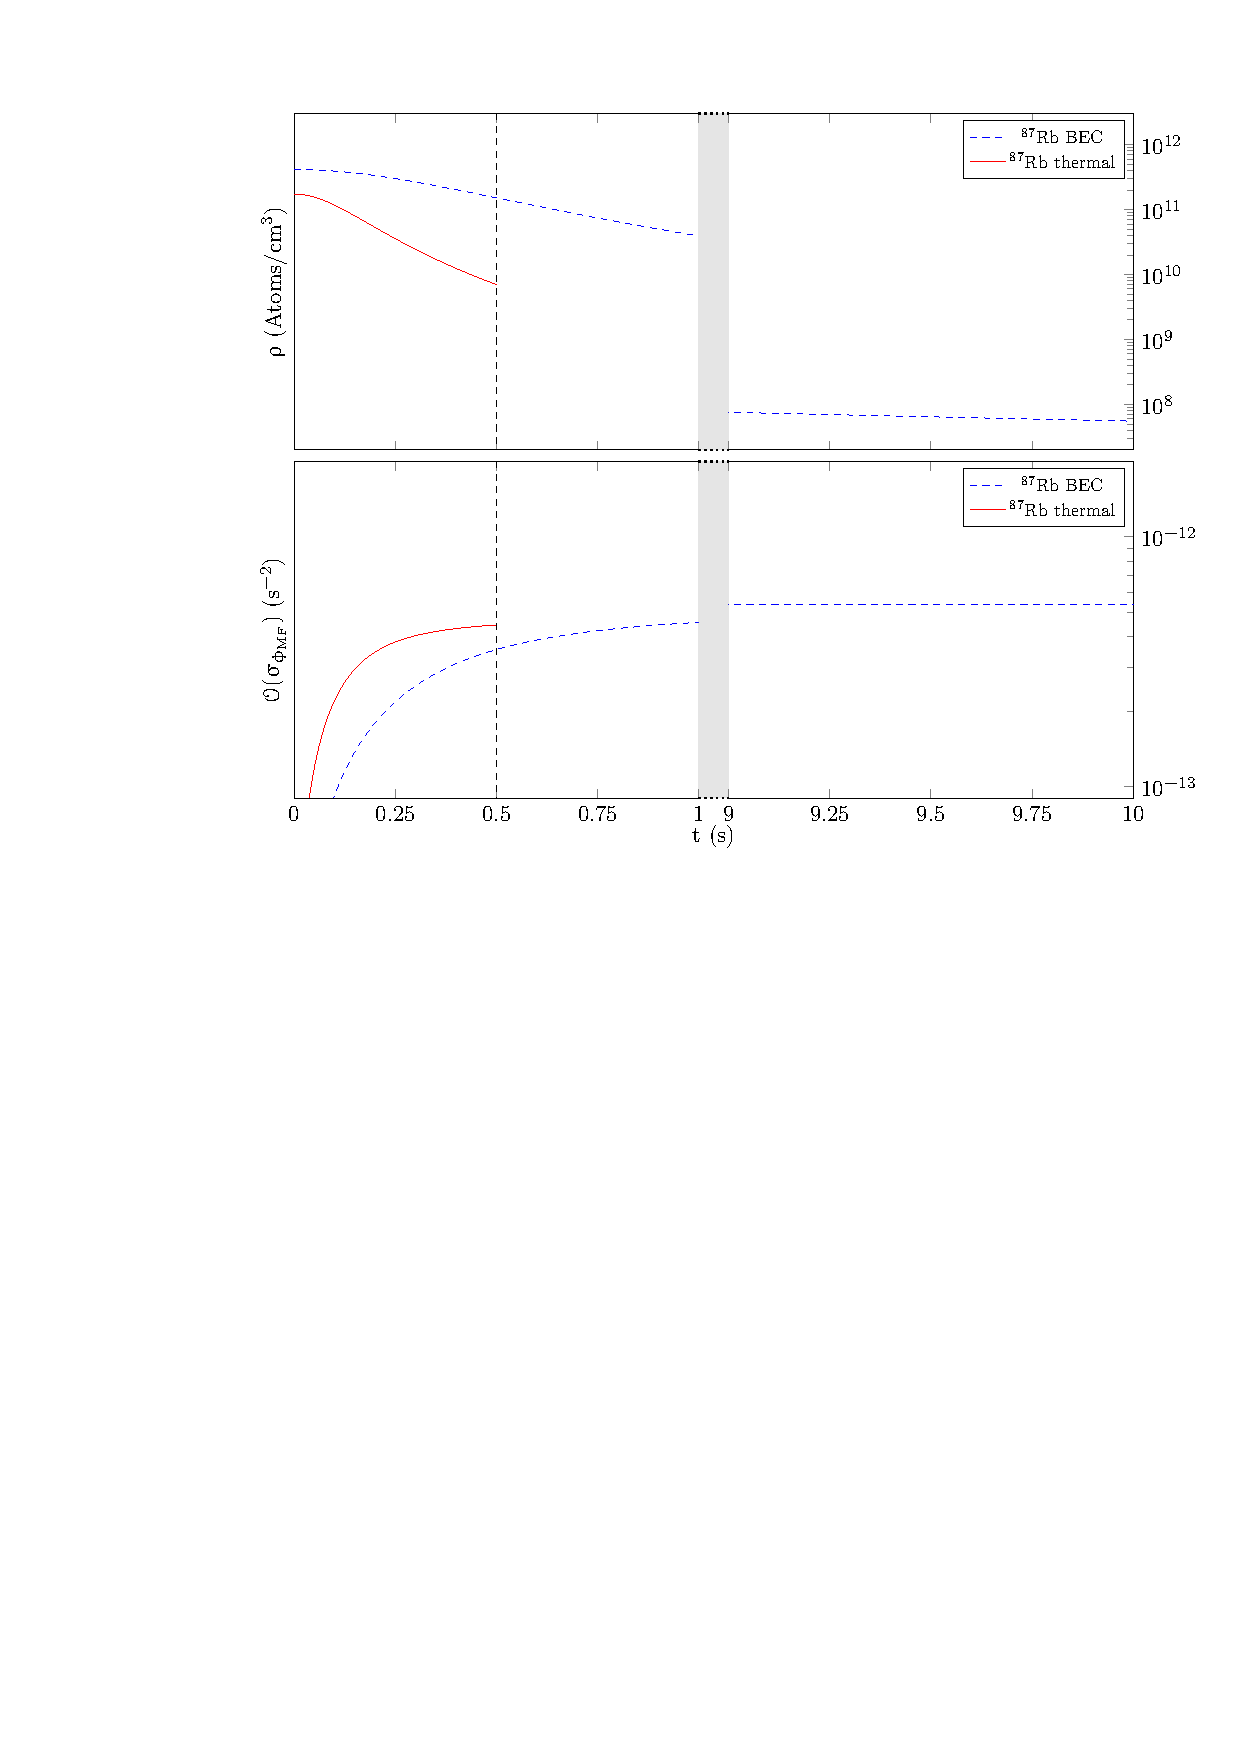
\includegraphics[width=\linewidth]{../MF-plot}
        }
    \caption{Atomic densities and time averaged mean-field statistical uncertainty for the space-gradiometer scenario described in \autoref{tab:numbers}. (a) Time-dependent density $\rho$ of the ensembles during the interferometer time based on the DKC sequence described in \autoref{tab:DKC}. (b) Fractional statistical phase uncertainty $\mathcal{O}(\sigma_{\phi_\text{MF}})$ due to mean-field effects according to equation \autoref{eq:MF} integrated over a number of $n_\text{cycle}$ experiments. }
    \label{fig:MF-effects}
\end{figure}

Assuming the same velocity spread for the two ensembles in the two interferometers and - as for the gravimeter case - the simplification of a constant curvature, the differential phase shift vanishes. Here, we drop this simplification and consider the propagation of a Gaussian beam which leads to a local dependency of the curvature, and thus to a non-vanishing phase shift in the differential signal. Assuming a residual radius of curvature of the retro-reflection mirror of 4\,km and a propagating the laser beam as outlined in \cite{Trimeche2019} introduces the differential phase shift as reported in~\autoref{tab:numbers}.
 
To reach the uncertainty goal of 2.5\,mE, an integration time on the order of 1 day is required in both cases. Albeit the high expansion rate of the thermal ensemble is accounted for with a shorter interrogation time of 0.5\,s (full cycle time of 1.2\,s), the shot noise uncertainty in the thermal case exceeds the one of the BEC case as the contrast drops to 33\% (97\% for the BEC after 10\,s).
Again, the WFA would hinder any further attempts for a better performance below the $10^{-12}\,s^{-2}$ level. All other systematic effects are complying with the performance required from this sensor and can be reduced by an increased number of verification shots. 

Being limited by WFA at the level of $4.4\times10^{-15}$, the BEC clearly leaves more room for improvement compared to thermal sources, which are bound three orders of magnitude above. Therefore, using a BEC source in this scenario is advantageous since it does neither suffer from a worse integration time nor a larger mean-field effect, yet significantly extends the desired sensitivity range compared to the thermal source.

\begin{figure}[h!]
    \centering
    %\subimport{GRAPHICS/}{AI-geometry-scheme.tex}
    \begin{tikzpicture}[declare function={
        f(\z,\v,\x) = \z+\v*\x-0.5*\g*\x^2;
        }
]
%
\begin{axis}[
    %title={Dual-species Mach-Zehnder atom interferometer},
    xlabel={t}, xlabel style={at={(1,0)}, anchor=west},
    ylabel={z (m)}, ylabel style={rotate=-90,at={(0,1)}, anchor=south},
    xmin=0.0, xmax=\tmin+\dtstart+2*\T+2*\dtmax,
    ymin=0, ymax=\zmax,
    axis lines = left,
    y=1.cm,
    x=1.cm,
    xtick={0,\tmin,\tmin+\dtstart,\tmin+\dtstart+\T,\tmin+\dtstart+\T+\T,\tmin+\dtstart+\T+\T+\dtmax},
    xticklabels={$0$,$t_\text{start}$,$t_0$,$t_0+T$,$t_0+2T$,$t_\text{end}$},
    ytick={0,1,...,12},
    legend pos=north west,
    %grid=both,
    ymajorgrids=true,
    grid style=dashed,
    ]
    %upper path
    \addplot[color=blue, samples=50, very thick][domain=\tmin:\tmin+\dtstart]{
        f(
        \zmin
        ,\vstart
        ,(x-\tmin)
        )
    };
    \addplot[color=blue, samples=50, very thick, dashed][domain=\tmin+\dtstart:\tmin+\dtstart+\T]{
        f(
            f(\zmin,\vstart,\dtstart)
            ,\vstart-\g*\dtstart+\keff
            ,x-\tmin-\dtstart
        )
    };
    \addplot[color=blue, samples=50, very thick][domain=\tmin+\dtstart+\T:\tmin+\dtstart+\T+\T]{
        f(
            f(f(\zmin,\vstart,\dtstart),\vstart-\g*\dtstart+\keff,\T)
            ,\vstart-\g*(\dtstart+\T)
            ,x-\tmin-\dtstart-\T
            )
    };
    %lower path
    \addplot[color=blue, samples=50, very thick][domain=\tmin+\dtstart:\tmin+\dtstart+\T]{
        f(
            f(\zmin,\vstart,\dtstart)
            ,\vstart-\g*\dtstart
            ,x-\tmin-\dtstart
        )
    };
    \addplot[color=blue, samples=50, very thick, dashed][domain=\tmin+\dtstart+\T:\tmin+\dtstart+\T+\T]{
        f(
            f(f(\zmin,\vstart,\dtstart),\vstart-\g*\dtstart,\T)
            ,\vstart-\g*(\dtstart+\T)+\keff
            ,x-\tmin-\dtstart-\T
        )
    };
    \addplot[color=blue, samples=50, very thick, dashed][domain=\tmin+\dtstart+2*\T:\tmin+\dtstart+\T+\T+\dtmax]{
        f(
            f(f(f(\zmin,\vstart,\dtstart),\vstart-\g*\dtstart,\T),\vstart-\g*(\dtstart+\T)+\keff,\T)
            ,\vstart-\g*(\dtstart+\T+\T)
            ,x-\tmin-\dtstart-\T-\T
        )
    };
    \addplot[color=blue, samples=50, very thick][domain=\tmin+\dtstart+2*\T:\tmin+\dtstart+\T+\T+\dtmax]{
        f(
            f(f(f(\zmin,\vstart,\dtstart),\vstart-\g*\dtstart,\T),\vstart-\g*(\dtstart+\T)+\keff,\T)
            ,\vstart-\g*(\dtstart+\T+\T)-\keff
            ,x-\tmin-\dtstart-\T-\T
        )
    };    
    %upper path
    \addplot[color=black, samples=50, very thick][domain=\tmin:\tmin+\dtstart]{
        f(
        \zmin
        ,\vstart+\dvstart
        ,(x-\tmin)
        )
    };
    \addplot[color=black, samples=50, very thick, dashed][domain=\tmin+\dtstart:\tmin+\dtstart+\T]{
        f(
            f(\zmin,\vstart+\dvstart,\dtstart)
            ,\vstart+\dvstart-\g*\dtstart+\keff
            ,x-\tmin-\dtstart
        )
    };
    \addplot[color=black, samples=50, very thick][domain=\tmin+\dtstart+\T:\tmin+\dtstart+\T+\T]{
        f(
            f(f(\zmin,\vstart+\dvstart,\dtstart),\vstart+\dvstart-\g*\dtstart+\keff,\T)
            ,\vstart+\dvstart-\g*(\dtstart+\T)
            ,x-\tmin-\dtstart-\T
            )
    };
    %lower path
    \addplot[color=black, samples=50, very thick][domain=\tmin+\dtstart:\tmin+\dtstart+\T]{
        f(
            f(\zmin,\vstart+\dvstart,\dtstart)
            ,\vstart+\dvstart-\g*\dtstart
            ,x-\tmin-\dtstart
        )
    };
    \addplot[color=black, samples=50, very thick, dashed][domain=\tmin+\dtstart+\T:\tmin+\dtstart+\T+\T]{
        f(
            f(f(\zmin,\vstart+\dvstart,\dtstart),\vstart+\dvstart-\g*\dtstart,\T)
            ,\vstart+\dvstart-\g*(\dtstart+\T)+\keff
            ,x-\tmin-\dtstart-\T
        )
    };
    \addplot[color=black, samples=50, very thick][domain=\tmin+\dtstart+2*\T:\tmin+\dtstart+\T+\T+\dtmax]{
        f(
            f(f(f(\zmin,\vstart+\dvstart,\dtstart),\vstart+\dvstart-\g*\dtstart,\T),\vstart+\dvstart-\g*(\dtstart+\T)+\keff,\T)
            ,\vstart+\dvstart-\g*(\dtstart+\T+\T)-\keff
            ,x-\tmin-\dtstart-\T-\T
        )
    };  
    \addplot[color=black, samples=50, very thick, dashed][domain=\tmin+\dtstart+2*\T:\tmin+\dtstart+\T+\T+\dtmax]{
        f(
            f(f(f(\zmin,\vstart+\dvstart,\dtstart),\vstart+\dvstart-\g*\dtstart,\T),\vstart+\dvstart-\g*(\dtstart+\T)+\keff,\T)
            ,\vstart+\dvstart-\g*(\dtstart+\T+\T)
            ,x-\tmin-\dtstart-\T-\T
        )
    };  
\end{axis}

    %create Laserbeams
    \draw[decorate, decoration = snake, very thick, red, opacity=0.5]
    ({\tmin + \dtstart},0) to ({\tmin + \dtstart},{.9*\zmax}) node[above] {$\pi/2$};
    \draw[decorate, decoration = snake, very thick, red, opacity=0.5,] 
    ({\tmin + \dtstart+\T},0) to ({\tmin + \dtstart + \T},{.9*\zmax}) node[above] {$\pi$};
    \draw[decorate, decoration = snake, very thick, red, opacity=0.5,] 
    ({\tmin + \dtstart + 2*\T},0) to ({\tmin + \dtstart + 2*\T},{.9*\zmax}) node[above] {$\pi/2$};
\end{tikzpicture}
    %\includegraphics[width=0.5\linewidth]{../AI-geometry-scheme}
    \caption{The geometry for a gradiometer consists of two MZ sequences that are operated simultaneously (black and blue lines). Each MZ sequence is formed by three consecutive light pulses that constitute a beam splitter (first $\pi/2$-pulse), a mirror ($\pi$-pulse) and a merging beam splitter after $2T$. The dashed lines indicate a change of the internal state due to a momentum transfer by the atom-light interaction. 
    A single MZ sequence corresponds to a gravimeter sequence to measure the coupling constant $g$ of the gravitational field to one species.
    Two MZ sequences operated with two different species allow for a determination of $\eta$. In this case the differential velocity at $t=t_\text{start}$ of the MZ sequences is set such that they spatially overlap to eliminate the gravity gradient, but remain sensitive to a potentially species specific differential acceleration.}
    \label{fig:AI-geometry-scheme}
\end{figure}
%
\subsection{WEP-test}\label{sec:WEP-test}
The WEP-test example is based on the parameters of the STE-QUEST satellite mission proposed in~\cite{Aguilera2014}. We here assume the test pair $^{41}$K and $^{87}$Rb. It aims at an Eötvös ratio $\eta$ determined with an uncertainty of $2\times10^{-15}$. As for the gradiometer, we compare a thermal ensemble at 0.5\,s of interrogation time (full cycle time of 0.83\,s) with a BEC at 10\,s (full cycle time of 20\,s) of interrogation time to ensure non-vanishing contrast and technically manageable ensemble sizes in both cases. In the last column of \autoref{tab:numbers}, the results of the comparison are displayed.

For the determination of the systematic effects one has to take into account the differences of the two atomic species such as the different expansion rates, atomic masses and initial conditions like spatial spread. The two different species-specific excitation rates are also evaluated and the minimum given in \autoref{tab:numbers}.

The effects of GGs and Coriolis force do not scale with $\sqrt{2}$ in this case, but rather with the mean square of two uncorrelated spreads (see \autoref{eq:mean-square-spreads}).
With two different species propagating in the arms, the mean-field effects are calculated as the mean-square sum of the individual mean-field effects of $^{87}$Rb and $^{41}$K as in \autoref{eq:MF}.
As for the gradiometer, one benefits from the differential suppression of WFA when matching the expansion rates of the ensembles~\cite{Aguilera2014}. As two different sources and two different species are used for the production of the ensembles, the systematic differential phase uncertainty is given by
\begin{equation}
    \delta_{\phi_\text{WFA}}= \frac{k_\text{eff}}{R} k_B \left(\frac{T_\text{at,K}}{m_\text{at,K}}-\frac{T_\text{at,Rb}}{m_\text{at,Rb}}\right)T^2,
\end{equation}
analogous to \autoref{eq:WFA}. 
By experimentally matching the velocity spreads of the two ensembles to the 20\% level in both arms, the WFA are suppressed by a factor of 3.

In the BEC case and in order for the statistical effects to be consistent with the mission performance goal, $10^6$ experimental cycles $n_\text{cycle}$ are needed. This leads to a full mission time on the order of five years in case of a highly elliptical orbit operation.
To reach the targeted uncertainty, an additional $10^6$ verification measurements $\nu_0$ are necessary. These measurements are included in the total mission time as they are performed on the transition between perigee and apogee parts of the orbit not dedicated to science measurements~\cite{Aguilera2014}. The contrast at the end of the sequence is at 99\% for both, $^{87}$Rb and $^{41}$K, and for the chosen set of parameters it is feasible to achieve the missions goals with condensed ensembles.

With a thermal ensemble, one would need an integration time on the order of $10^8$ s to suppress mean-field effects, and $10^6$ verification shots to estimate the phase uncertainty due to GGs and the Coriolis effect to a sufficient level. Moreover, even for the reduced interrogation time of 0.5 s, the contrast is at 43\% and the shot noise is almost 6 times larger than in the BEC case.

We conclude that - for the chosen set of parameters - it is possible to achieve the mission goals with condensed ensembles. The thermal case is, however, limited to the $10^{-12}$ level due to the WFA effects stemming from the large expansion rates of the thermal ensembles~\cite{Karcher2018}. In order to reach a reduced velocity spread with a thermal ensemble comparable to that of a BEC, the DKC would be required to handle ensembles with a diameter on the order of 0.5\,m after a pre-lens free expansion time of several seconds. As for the space-gradiometer, this is unpractical for obvious manipulation and excitation reasons. In the condensed regime, a simultaneous collimation of the dual-source was recently considered in reference~\cite{Corgier2020} and shown to be feasible.
%\end{document}